\chapter{Métodos de Funciones Valor}%
\label{cha:value_function_methods}

\lecture{7}{2020-06-15}{Value Function Methods}

\section{Usando solamente un crítico, sin un actor}%
\label{sec:usando_solamente_un_crítico_sin_un_actor}

Los algoritmos basados en Policy Gradient suelen tener una varianza alta. Para contrarrestarlo se
introducen \textit{baselines} y un crítico. Se puede pensar que para deshacernos de la
varianza completamente se puede eliminar el actor.

Esto se tiene que hacer en la definición del \textit{advantage} $A^\pi(s_t,a_t)$. Se pueden
escoger las accioens siguiendo la política $\pi = arg\max_{a_t} A^\pi(s_t,a_t)$. En este
caso, la política será al menos tan buena como cualquier $a_t\sim\pi(a_t,s_t)$ a no
ser que $\pi$ sea la mejor política posible.

\begin{align}
    \label{eq:detpol}
    \pi'(a_t|s_t) = \begin{cases}
        1 \text{ si } a_t = arg\max_{a_t}A^\pi(s_t,a_t)\\
        0 \textrm{ en cualquier otro caso }
    \end{cases}
\end{align}

\begin{figure}[htpb]
	\centering
	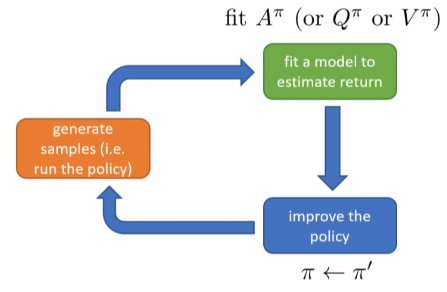
\includegraphics[width=0.5\linewidth]{figures/2020-06-15-110004_447x292_scrot.png}
\end{figure}

Para entender estos métodos, se tiene que introducir el concepto de iteración de la política:

\begin{algorithm}
    \caption{Policy Algorithm}
    \While{se entrene}{
        Evaluar $A^\pi(s,a)$\\
        $\pi \gets \pi'$ \\
    }
\end{algorithm}

Como antes, el \textit{advantage} sigue siendo:
\begin{align}
    \label{eq:advantage}
A ^ { \pi } ( s , a ) = r ( s , a ) + \gamma E [ V ^ { \pi } ( s ^ { \prime } ) ] - V ^ { \pi } ( s )
\end{align}

Para calcular $A^\pi(s,a)$, se tiene que estimar primero  $V^\pi$. Para estimarlo se puede usar
Programación Dinámica.

\subsection{Programación Dinámica}%
\label{sub:programación_dinámica}

Se asume que se conoce $p(s'|s,a)$, y  $s$ y $a$ son ambos discretos y pequeños.

Como ejemplo, se propone un mundo con 16 estados, 4 acciones (moverse en las direcciones). Por lo que se puede guardar
$V^\pi$ en una tabla.  $T$ será un tensor de 16x16x4.

\begin{figure}[htpb]
	\centering
	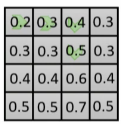
\includegraphics[width=0.15\linewidth]{figures/2020-06-15-110633_121x124_scrot.png}
\end{figure}

Para estimar los valores de los estados, se utiliza la técnica llamada \textit{bootstrapped
update}, que consiste en:
\begin{align}
V ^ { \pi } ( s ) \leftarrow E _ { a \sim \pi ( a | s ) } [ r ( s , a ) + \gamma E _ { s ^ { \prime } \sim p ( s ^ { \prime } | s , a ) } [ V ^ { \pi } ( s ^ { \prime } ) ] ]
\end{align}

Donde en $V^\pi(s')$ se usa la estimación que se tenga en ese momento.

Como se usa una política determinista (ecuación \ref{eq:detpol}), se puede expresar la política
como $\pi(s)=a$, por lo que el \textit{bootstrapped update} queda simplificado a:

\begin{align}
V ^ { \pi } ( s ) \leftarrow r ( s , \pi ( s ) ) + \gamma E _ { s ^ { \prime } \sim p ( s ^ { \prime } | s , \pi ( s ) ) } [ V ^ { \pi } ( s ^ { \prime } ) ]
\end{align}

En MDP totalmente observables (se tiene el estado en vez de una observación) siempre existe
una política determinista que es mejor que cualquier otra política. En el caso de los MDP
parcialmente observables esto deja de ser cierto.

\subsubsection{Simplificación}%
\label{ssub:simplificación}

Partiendo de la ecuación \ref{eq:detpol}, y viendo la definición de $A^\pi(s,a)$ en la ecuación
\ref{eq:advantage}, se concluye que
$arg\max_{a_t}A^\pi(s_t,a_t)=arg\max_{a_t}Q^\pi(s_t,a_t)$ ya que el único término de
$A^\pi(s,a)$ que depende de  $a$ es $r(s,a)$. Esto es de interés porque:
\begin{align}
Q ^ { \pi } ( s , a ) = r ( s , a ) + \gamma E [ V ^ { \pi } ( s ^ { \prime } ) ]
\end{align}

Que es una expresión más sencilla que la anterior.

\begin{algorithm}
    \caption{Value Iteration simplificado}
    \While{$V(s)$ no converja}{
        $Q(s,a)\gets r(s,a)+\gamma E[V(s')]$\\
        $V(s)\gets \max_a Q(s,a)$
    }
\end{algorithm}

\begin{figure}[htpb]
	\centering
	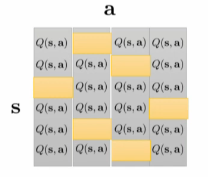
\includegraphics[width=0.2\linewidth]{figures/2020-06-15-113002_208x177_scrot.png}
    \caption{Se guardan todos los valores de Q(s,a) en una tabla. Los valores V(s) se
    corresponderán a los máximos por cada fila.}
\end{figure}

\subsection{Fitted Value Iteration}%
\label{sub:fitted_value_iteration}

La programación dinámica no se puede aplicar a problemas reales por culpa de la maldición de la
dimensionalidad, por lo que se puede intentar usar una red neuronal para estimar las funciones de valores.

Se tiene una red neuronal $V:S\mapsto \R$, donde  $\phi$ son sus parámetros, y se entrena con
el siguiente objetivo:
 \begin{align}
L ( \phi ) = \frac { 1 } { 2 } \| V _ { \phi } ( s ) - \operatorname { max } _ { a } Q ^ { \pi } ( s , a ) \| ^ { 2 }
\end{align}

\begin{algorithm}
    \caption{Fitted value iteration}
    \label{alg:q-fit}
    \While{$V(s)$ no haya convergido }{
        $ y _ { i } \leftarrow \operatorname { max } _ { a _ { i } } ( r ( s _ { i } , a _ { i } ) +
        \gamma E [ V _ { \phi } ( s _ { i } ^ { \prime } ) ] ) $\\
        $ \phi \leftarrow \operatorname { arg } \operatorname { min } _ { \phi } \frac { 1 } { 2 } \sum _ { i } \| V _ { \phi } ( s _ { i } ) - y _ { i } \| ^ { 2 } $
    }
\end{algorithm}

Se tiene que reformular el problema para que la red neuronal no reciba todos los posibles
estados, ya que estos pueden crecer exponencialmente con el tamaño del problema.

Todavía se asume que se conoce $p(s'|s,a)$.

Para deshacerse de la necesidad de enumerar todos los estados, se pueden muestrear
un subconjunto.

Para deshacerse de la necesidad de conocer la dinámica de transición $p(s'|s,a)$ se
puede cambiar el primer paso de \textit{policy iteration}. Donde antes se iteraba:
\begin{align}
V ^ { \pi } ( s ) \leftarrow r ( s , \pi ( s ) ) + \gamma E _ { s ^ { \prime } \sim p ( s ^ { \prime } | s , \pi ( s ) ) } [ V ^ { \pi } ( s ^ { \prime } ) ]
\end{align}

Ahora pasará a iterarse $Q$ directamente:
\begin{align}
Q ^ { \pi } ( s , a ) \leftarrow r ( s , a ) + \gamma E _ { s ^ { \prime } \sim p ( s ^ { \prime } | s , a ) } [ Q ^ { \pi } ( s ^ { \prime } , \pi ( s ^ { \prime } ) ) ]
\end{align}

Por lo que ahora se guarda un valor por cada par estado-acción en vez de solo de por cada
acción. La esperanza puede estimarse mediante muestras.

En el algoritmo \ref{alg:q-fit} hay una maximización escondida en $E[V_\phi(s'_i)] \approx
\max_{a'}Q_\phi(s'_i,a'_i)$. Pero esta maximización no requiere de conocer las probabilidades de
transición, ya que solo se tienen que probar las acciones en el aproximador de funciones (red
neuronal). En el caso de que las acciones sean contínuas, para encontrar la $a'$ que maximice
la  $Q$ se tiene que plantear un problema de optimización.

Este método funciona incluso para muestras \textit{off-policy}, y solo se necesita una red
neuronal. Como desventaja, se pierden las garantías de convergencia.

\begin{algorithm}
    \caption{Fitted Q-Iteration}
    \KwIn{K: Número de veces que se entrenará con un mismo dataset}
    \KwIn{N: Tamaño del dataset}
    \KwIn{S: Número de pasos del gradiente}
    \While{se siga entrenando}{
        Crear un dataset $\{(s_i,a_i,s'_i,r_i)\}$ usando una política\\
        \While{Repetir $K$ veces}{
            Se crean los targets usando  \textit{bootstrapping}: $y_i\gets r(s_i,a_i) +
            \gamma\max_{a_i'}Q_\phi(s'_i,a'_i)$ \\
            Regresión: $\phi\gets arg\min_\phi \frac{1}{2}\sum_i ||Q_\phi(s_i,a_i)-y_i||^2$
        }
    }
\end{algorithm}

La razón por la que está el bucle exterior es que la política inicialmente puede ser
bastante mala y no explorar todos los valores.

En el paso final, se está minimizando el error de Bellman:
\begin{align}
\epsilon = ||Q_\phi(s_i,a_i)-y_i||^2 = \frac { 1 } { 2 } E _ { ( s , a ) \sim \beta } [ ( Q _ { \phi } ( s , a ) - [ r ( s , a ) + \gamma \operatorname { max } _ { a ^ { \prime } } Q _ { \phi } ( s ^ { \prime } , a ^ { \prime } ) ] ) ^ { 2 } ]
\end{align}

Pero en los otros dos pasos esto no es así (incluso en el paso 2, se incrementa el error de
Bellman). Cuando el error de Bellman es 0,
$Q_\phi(s,a)=r(s,a)+\gamma\max_{a'}Q_\phi(s',a')$.

Malas noticias: no se sabe realmente lo que se está optimizando con este algoritmo.

\section{Q-Learning}%
\label{sec:q_learning}

\subsection{Online Q-Learning}%
\label{sub:online_q_learning}

\begin{algorithm}
    \caption{Fitted Q-Iteration}
    \While{se siga entrenando}{
        Tomar una acción $a_i$ y observar  $(s_i,a_i,s_i',r_i)$.\\
         $y_i\gets r(s_i,a_i) + \gamma\max_{a_i'}Q_\phi(s'_i,a'_i)$ \\
         $\phi\gets\phi-\alpha \frac{dQ_\phi}{d\phi}(s_i,a_i)(Q_\phi(s_i,a_i)-y_i)$
    }
\end{algorithm} 

El paso 1 sigue siendo \textit{off-policy} por lo que se puede usar cualquier política. Para el
caso de aproximadores de funciones, no es buena idea entrenar con un batch de tamaño 1 ya que
eso genera inestabilidad.

\subsection{Exploración con Q-Learning}%
\label{sub:exploración_con_q_learning}

Para el paso 1 del algoritmo anterior, se puede usar la política de la ecuación \ref{eq:detpol}.
Esta política inicialmente puede ser mala ya que al ser determinista puede ser que no
se llegue a ciertos estados necesarios para resolver el problema.

Hay varias formas de arreglar esto. Una de ellas es \textit{epsilon-greedy}, donde la política
pasa a ser:
\begin{align}
    \pi(a_t|s_t)= \begin{cases}
        1-\epsilon \textrm{ si } a_t = arg\max_{a_t} Q_\phi(s_t,a_t)\\
        \frac{\epsilon}{|A|-1} \textrm{ en caso contrario }
    \end{cases}
\end{align}

Otra forma de solucionar esto es la llamada exploración de Boltzmann. La transformación
a aplicar tiene que mapear cada valor a un número positivo, la exponencial suele funcionar
bien. Este método tiende a alejar el agente de las decisiones de las que está muy seguro. Si
un valor de Q es muy bajo, es muy improbable que lo coja. También puede ser mejor aplicarlo
cuando el espacio de acciones es grande.
\begin{align}
    \pi(a_t|s_t)\propto \exp(Q_\phi(s_t,a_t))
\end{align}
